% ValueRTS: ISSTA 2027 submission draft, generated from the paper draft doc on 26 Nov 2026.
% Red [..] marks are placeholders, filled after the 13 Dec run freeze.
\documentclass[acmsmall,screen,review,anonymous]{acmart}
\usepackage{booktabs}
\usepackage{tabularx}
\usepackage{listings}
\usepackage{xcolor}
\usepackage{xspace}
\usepackage[most]{tcolorbox}
\usepackage{enumitem}
\setlist[itemize,enumerate]{leftmargin=*,topsep=2pt,partopsep=0pt,itemsep=1pt,parsep=0pt}
\lstset{basicstyle=\ttfamily\small,columns=fullflexible,keepspaces=true,frame=single,showstringspaces=false}
\newcommand{\ph}[1]{\textcolor{red}{[#1]}}
% Style conventions (as in recent ISSTA/ICSE/ASE RTS papers):
% - the tool's name through one macro, in plain text like NameRTS and BabelRTS;
% - run-in paragraph headings in bold sentence case ending with a period, through one macro;
% - italics only for a term at its definition and for the key insight; no bold inside sentences;
% - research questions as a list with bold labels; each RQ ends with a shaded "Answer to RQn" box.
\newcommand{\tool}{ValueRTS\xspace}
\newcommand{\para}[1]{\smallskip\noindent\textbf{#1}\hspace{0.4em}}
\newtcolorbox{answerbox}[1]{enhanced,breakable,colback=black!5,colframe=black!45,boxrule=0.5pt,arc=1.5pt,
  left=5pt,right=5pt,top=3pt,bottom=3pt,fontupper=\small,before skip=6pt,after skip=6pt,
  title={\textbf{Answer to RQ#1}},coltitle=black,attach title to upper={:\ }}

\setcopyright{none}
\acmConference[ISSTA 2027]{ACM SIGSOFT International Symposium on Software Testing and Analysis}{2027}{}

\begin{document}

% Title chosen 26 Nov 2026; confirm with Dr Li (it cannot change after submission).
\title{ValueRTS: Safe Regression Test Selection for AI Coding Agents in Python}
\author{Anonymous Author(s)}
\affiliation{\institution{Anonymous Institution}\country{Anonymous}}

\begin{abstract}
Nowadays, AI coding agents often rely on the project's tests to check their changes,  they rarely run the whole suite, and the tests they skip are where their regressions hide. Regression test selection (RTS) runs only the tests a change can affect, but Python RTS tools are blind to a central part of Python programs: the state a package builds when it is imported, such as lookup tables, registries and constants. Coverage-based tools credit this code to no test, and static, name-based tools either link it to every test or miss it.

We present \tool, an RTS technique for Python that compares import-time state across versions. \tool records each test's execution once, fingerprints the values a package builds at import, and after a change selects the tests whose recorded execution ran changed code, used a changed value, or read a changed file. It credits shared execution, such as fixture set-up, to every test that relies on it.

We evaluate \tool on \ph{B1: N} consecutive real commits from 20 Python projects, including the 500 commits of NameRTS's benchmark, on \ph{B1b: N} real bugs obtained by reversing SWE-bench fixes, and on \ph{B3: N} regressions introduced by published AI agents. \tool misses a failing test on \ph{B1: X\%} of failure-inducing changes, against \ph{B1: Y\%} for NameRTS and \ph{B1: Z\%} for pytest-testmon, while running \ph{B1: T\%} of the suite's test time. On agent regressions it misses \ph{B3: X\%} of broken tests against \ph{B3: Y\%} for NameRTS. \ph{B4: one sentence on agents in the loop, or omit.}
\end{abstract}

\begin{CCSXML}
<ccs2012>
<concept><concept_id>10011007.10011074.10011099.10011102.10011103</concept_id>
<concept_desc>Software and its engineering~Software testing and debugging</concept_desc>
<concept_significance>500</concept_significance></concept>
</ccs2012>
\end{CCSXML}
\ccsdesc[500]{Software and its engineering~Software testing and debugging}
\keywords{regression test selection, Python, import-time state, AI coding agents}

\maketitle

\section{Introduction}\label{sec:introduction}
AI coding agents such as Claude Code, Codex and Cursor now change real code bases with little supervision, and they rely on the project's tests to check their work. Across 7,745 public SWE-bench trajectories, agents ran the test framework 8.8 times per task on average, and forbidding test execution cut Claude Code's time by about half and its tokens by about 60\%~\cite{lin2026runornot}. In industry, Anthropic reports a 25-fold increase in CI jobs over six months, with Claude now authoring about 80\% of the code its engineers ship~\cite{malhotra2026ci}.

Running every test is rarely an option. SWE-bench tasks come with 9,012 tests on average in SWE-bench Lite and 11,769 in SWE-bench Verified, and a full run takes about 24 minutes on average~\cite{chen2026oldtests}. Agents therefore run a few tests they judge relevant; even the benchmark that grades them runs only the tests in the files edited by the task's test patch, about 121 tests per task~\cite{jimenez2024swebench}. Agents also often stop without re-checking their final edit: in 61.8\% of 2,500 SWE-bench Verified runs, no validation command followed the last source edit within the agent's final five actions~\cite{shu2026resolve}. Breakage elsewhere therefore goes unseen. Of \ph{B3: 42,116} patches that published SWE-bench agents submitted on eight pure-Python repositories, at least \ph{B3: 16.4\%} broke a test in SWE-bench's own lists that passed before the patch; in \ph{B3: 159} of these regressions that we ran against the full suite, \ph{B3: 97\%} of the broken tests lay outside those lists.

Regression test selection (RTS) addresses this trade-off: given a change, run only the tests the change can affect~\cite{yoo2012survey}. An RTS technique is \emph{safe} if no test it skips can be affected by the change~\cite{gligoric2015ekstazi}. For Java, safe RTS is mature: Ekstazi records the classes and files each test depends on, and credits a class's static initialiser to every test that uses the class, not only to the first~\cite{gligoric2015ekstazi}. For Python it is not, because of what happens when a package is imported. Python runs every top-level statement of a module at import, before any test starts, and stores the results in values that tests read later: lookup tables, registries, dispatch tables, constants. In \ph{RQ1: 61\%} of real commits, and \ph{RQ1: 78\%} of commits that break a test, the change alters such import-time statements.

Existing Python RTS handles this state either coarsely or not at all. Coverage-based tools such as pytest-testmon record the lines each test executes; import-time code executes before any test starts and is credited to none, and testmon's own test suite marks a changed import-time constant as a known miss~\cite{testmon}. NameRTS~\cite{wang2026namerts}, which outperforms the previous state of the art, BabelRTS, follows names statically and puts names accessed during import under a shared key, so they are ``treated as reachable to all test files''. Names built at run time and entries of lookup tables can escape it (Section~\ref{sec:results}). Linking every test to all import-time code is safe but runs \ph{RQ2: T\%} of the suite's test time. No technique checks whether the import-time state a test depends on actually changed.

We present \tool, an RTS technique for Python built on one key insight: \emph{compare the values a package builds at import across versions, and link only the changed values to the tests that use them}. \tool records each test's execution once, under Python 3.12's low-overhead monitoring, each test file in a fresh process. It fingerprints every module-level value and class attribute, in a form stable across runs. After a change it selects the tests that ran changed code, ran code that names a changed value, or read a changed file. Fixture set-up and cached results are credited to every test that relies on them, not only to the first. Where no dependency can be established, \tool runs more tests rather than fewer.

We evaluate \tool against pytest-testmon, NameRTS, EkstaP, TDAD and the traditional rule of selecting every test that executes changed code, on four benchmarks: \ph{B1: 1,000} consecutive real commits from 20 projects, including all 500 commits of NameRTS's benchmark scored with NameRTS's own metric; \ph{B1b: 500} real bugs obtained by reversing SWE-bench fixes; \ph{B3: N} regressions that published agents introduced on SWE-bench, with a full-suite ground truth; and \ph{B4: scope} agent runs with \tool in the loop. \tool and every baseline were frozen before any run, and 6 of the 20 projects were never used during development. \tool misses a failing test on \ph{B1: X\%} of failure-inducing commits, against \ph{B1: Y\%} for NameRTS and \ph{B1: Z\%} for testmon, at \ph{B1: T\%} of test time. On changes that touch import-time state, the gap is \ph{RQ1: ...}.

In summary, this paper makes the following contributions:

\begin{itemize}
  \item We propose, to our knowledge, the first RTS technique that compares, across versions, the program state a package builds at import and links the changed values to the tests that use them. Unlike uRTS~\cite{wang2023urts} it needs no configuration API, and unlike PolDet~\cite{gyori2015poldet} it compares state across versions rather than between tests in one run.
  \item We record shared execution per test, crediting fixture set-up and cached readers to every test that relies on them, which coverage-based Python tools do not.
  \item We implement \tool, an open-source RTS tool for pytest that combines these with established practice (a fresh process per test file, as in NameRTS; file dependencies, as in Ekstazi) and runs as a finish check for coding agents.
  \item We evaluate six tools on real history, real bugs and real agent regressions, in one frozen setup with held-out projects, and report missed failures and the classic safety measure side by side.
  \item We release \ph{B3: N} real agent regressions from published SWE-bench agents, reproduced with a full-suite ground truth.
\end{itemize}


\section{Background and motivating example}\label{sec:background-and-motivating-example}
\para{Tests in pytest.}A pytest suite is a set of test files. pytest imports each file to \emph{collect} its tests, and in doing so imports the package under test. Fixtures supply set-up to tests; a fixture with a module, class or session scope runs once and is shared by every test that uses it. Tests may also be generated at collection time from data (\texttt{parametrize}). All of this runs before, or outside, any single test.

\para{Import-time state.}Importing a Python module runs every top-level statement and every class body in it. Packages use this to build the values the rest of the code reads: dialect and token tables, plugin registries, dispatch tables, compiled patterns, constants. The example below is illustrative and simplified from the pattern we see in sqlglot's dialects and pygments' lexers.

\begin{lstlisting}[language=Python]
# formats.py: runs once, when the package is imported
def _iso(value): ...
def _us(value): ...
FORMATS = {"iso": _iso, "us": _us}      # built at import

# render.py
def render(value, style):
    return FORMATS[style](value)        # reads the table at run time

# test_render.py
def test_us(): assert render(D, "us") == "12/31/2026"
def test_iso(): assert render(D, "iso") == "2026-12-31"
\end{lstlisting}

Suppose a change maps \texttt{"us"} to a different function. \texttt{render} is unchanged, and so is every function a test calls by name, yet \texttt{test\_us} now fails. A tool that decides from changed code sees only a changed module-level statement. A tool that decides from changed \emph{values} sees that \texttt{FORMATS["us"]} changed, finds \texttt{render} as the code that reads \texttt{FORMATS}, and selects the tests whose recorded execution ran \texttt{render}: both tests here, and none of the suite's tests that never render.

\para{Why existing tools miss it.}Coverage-based tools record which lines ran during each test. The statement that builds \texttt{FORMATS} ran during collection, credited to no test, so a change to it selects nothing (testmon; Section~\ref{sec:related-work}). NameRTS follows names statically: it sees that \texttt{render} names \texttt{FORMATS}, but it puts names used at import under a key shared by all tests, so changing the table selects every test, and a table indexed by a string built at run time is followed by no name at all. Selecting every test that executed changed code is safe here only because every test executed the import, which again selects everything.

\para{Shared and cached execution.}The same blind spot appears whenever work is done once and reused. A module-scoped fixture's set-up is credited by coverage tools to the first test that uses it; a cache filled on first use is credited to the first test that fills it. In both cases later tests depend on code that their own recording does not show. We observed testmon rerun only the first of two tests broken by a change to a shared fixture's helper (Section~\ref{sec:results}).


\section{Approach}\label{sec:approach}
\tool follows three principles: record everything a test depends on; judge import-time changes by the values tests use; and when a dependency cannot be established, run more tests rather than fewer. It works in four steps (Figure~\ref{fig:overview}): \emph{record} once at a base commit, \emph{snapshot} the import-time state, \emph{compare} after each change, and \emph{select}.

\begin{figure}[t]
\centering
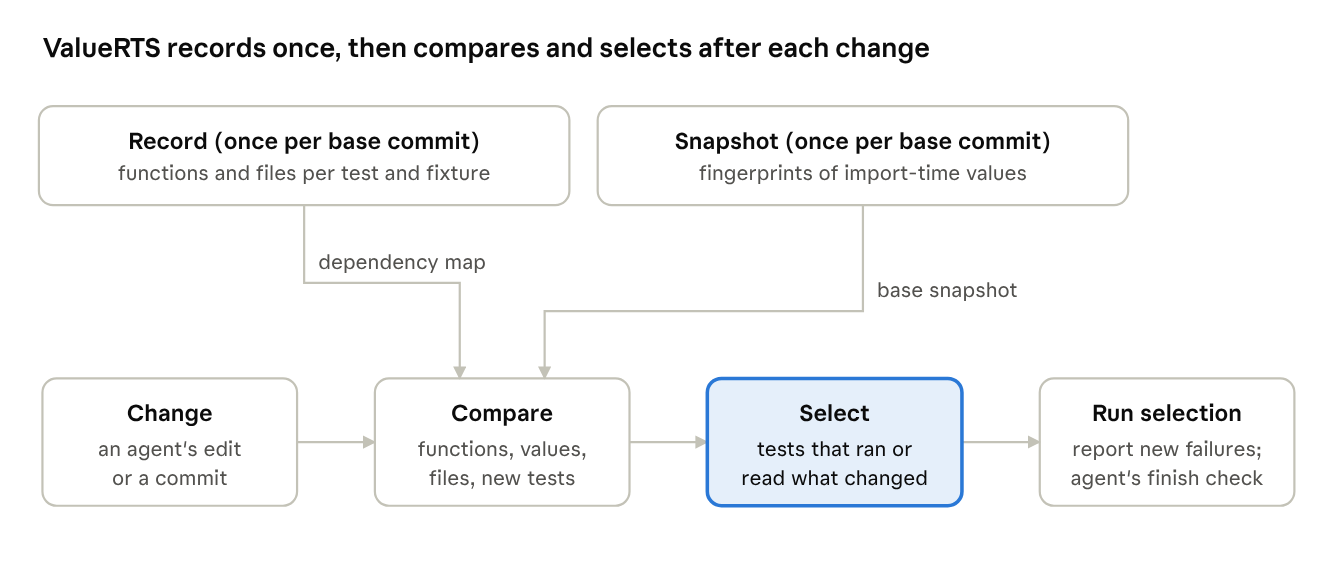
\includegraphics[width=\linewidth]{figures/overview.png}
\caption{\tool end to end. Recording and the base snapshot happen once per base commit; every later change is compared against them, and only the selected tests run before the agent can finish.}
\label{fig:overview}
\end{figure}


\subsection{Challenges}
Selecting few tests in Python without missing failures raises five challenges.

\begin{itemize}
  \item \textbf{C1:} \emph{Detecting import-time changes.} The values a package builds at import are arbitrary objects (functions, classes, closures, large tables), and some come out in a different order on each run: sympy's dispatch tables are ordered by memory address. Comparing them must be stable, so that run-to-run noise is not mistaken for a change.
  \item \textbf{C2:} \emph{Linking changed values to tests.} Tests read values through names and attributes, not calls, so a record of the functions each test ran does not show them. Code that reads a value often runs once and caches its result, so later tests reach it only through the cache.
  \item \textbf{C3:} \emph{Execution shared between tests.} A module-scoped fixture runs once for all its users, and a cache is filled by whichever test runs first. Coverage tools credit both to the first test only.
  \item \textbf{C4:} \emph{Dependencies outside Python code.} Tests read JSON data, templates, expected outputs and configuration, sometimes while pytest collects or parametrises tests, and some \texttt{.py} files are read as data rather than executed.
  \item \textbf{C5:} \emph{Precision must cost less than it saves.} Finer analysis selects fewer tests but costs more per change: method-level static RTS has been measured at 695\% of the time of running all tests~\cite{legunsen2016static}. Deciding whether import-time state changed requires importing two versions of the package and fingerprinting every module-level value, about 57,000 in sympy.
\end{itemize}


\subsection{Record (C3, C4)}
\tool runs the suite once at a base commit with a pytest plugin built on Python 3.12's low-overhead monitoring (PEP 669). The first time a project function starts within a recording target, the plugin stores its key (file and first line) for that target and switches the event off for it until the target changes. Methods stay on, so the classes of the objects they run on are recorded too. Audit hooks (PEP 578) record the project files each test opens and the directories it lists.

A recording target is a test, a fixture instance, or the package import. Fixture set-up is recorded once per fixture instance and credited to every test that uses that instance, so a shared fixture's code belongs to all its users (C3). Code that runs while a package module is imported at start-up is kept apart from every test, in a global record, and is handled by the snapshot. Each test file runs in a fresh interpreter, so one file's imports and caches cannot hide another file's dependencies. Tests that start subprocesses, or whose set-up fails, cannot be recorded completely and are always selected.


\subsection{Snapshot (C1)}
\tool imports the package at the base commit and, after a change, at the working tree, each in a separate process, and fingerprints every module-level value and class attribute. Plain data is fingerprinted by value, functions by a hash of their code (so a changed lambda inside a table counts), and other objects by type and attributes, with memory addresses stripped, following PolDet's abstraction of heap state~\cite{gyori2015poldet}. Sets and dictionaries are compared regardless of order. The base snapshot is taken in nine samples; a value whose fingerprint differs between samples is compared without order, and if it still differs it is treated as unstable rather than changed.


\subsection{Compare (C1, C2, C4)}
After a change, \tool finds:

\begin{itemize}
  \item \emph{changed functions}, from the changed lines of the diff and by comparing each function's code by name, which catches edits that a line diff credits to the wrong function; edits that only touch docstrings or formatting are ignored;
  \item \emph{changed import-time values}, by comparing the two snapshots, but only when the change touches code that runs at import;
  \item \emph{changed files}, from the diff;
  \item \emph{new tests}, which are always run.
\end{itemize}

For each changed value, \tool finds the functions that name it, through an index of the names each function uses, then follows the names assigned from it and the callers of those functions, so that a reader whose result was cached is still linked to every test that reaches it (C2).


\subsection{Select (C5)}
\tool selects every test whose recording, own or through its fixtures, ran a changed function, ran a function linked to a changed value, or read a changed file. A file read while tests were collected selects its whole test file; one read during the package import selects every test. Where no dependency can be established, it runs the full suite: a changed pytest configuration, a file that no longer parses, a changed non-Python file no test was seen to read, or a map recorded at a commit outside the current history. When the edited functions alone already reach 90\% of the suite's test time, \tool runs the full suite directly rather than spend time selecting. The snapshot is taken only when a change touches import-time code, so most selections take a few seconds (Section~\ref{sec:results}, RQ4).


\section{Implementation}\label{sec:implementation}
\tool is a Python package and a pytest plugin, \ph{LOC: N} lines, for Python 3.12 or later. The recorder uses \texttt{sys.monitoring} and audit hooks only; it needs no change to the project or its tests.

\para{Recording speed.}Recording forks each test file's process from one interpreter that has already imported pytest, shares compiled bytecode between the processes of one recording, and starts the longest test files first. None of this changes the recorded map: on sqlglot and pygments the maps are identical to those of a fresh interpreter per file, except for tests that draw random inputs, which differ between any two recordings. \ph{Check on the other three projects before the freeze.}

\para{Agent integration.}\tool runs inside Claude Code through its hooks. When the agent runs a broad test command, \tool replaces it with the selected tests and reports only failures that are new since the base commit; when the agent says it is done, \tool runs the selected tests as a finish check. The map is recorded once per task, before the agent starts.

\para{Use of generative AI.}Following ACM's policy on authorship, we disclose that \tool's implementation, the experiment harnesses and the analysis scripts were written with the help of an AI assistant (Claude, Anthropic). Every component was checked by us: \tool by \ph{N} unit tests over small synthetic projects and by maps compared across recording modes; the harnesses by dry runs on real commits and by checking every reported miss against a rerun of the tests; and every miss of every tool by manual root-cause analysis. The agent study uses Claude Code as its subject, as described in Section~\ref{sec:evaluation-setup}.


\section{Evaluation setup}\label{sec:evaluation-setup}

\subsection{Research questions}
We answer four research questions.

\begin{description}
  \item[RQ1 (Effectiveness):] How often does each tool miss a failing test on real changes, and at what cost? We split the results by whether the change touches import-time state.
  \item[RQ2 (Ablation):] What does each part of \tool contribute, and what does the traditional rule cost?
  \item[RQ3 (AI agents):] Does each tool select the tests that AI agents actually break, and does \tool in the loop change agent outcomes, time or cost?
  \item[RQ4 (Overhead):] What do recording and selection cost, and when does recording pay for itself?
\end{description}

RQ1 uses B1 and B1b, with B2 as a secondary benchmark for change kinds; RQ2 uses B1 and B2; RQ3 uses B3 and B4; RQ4 uses B1 and B1b.


\subsection{Benchmarks}
\begin{itemize}
  \item \textbf{B1:} \emph{Real history.} 20 Python projects: the 10 of NameRTS's benchmark, the 4 we used during development (sqlglot, pygments, SQLAlchemy, datasette) and 6 held-out projects never used during development \ph{list}. For NameRTS's projects we use its own 500 published commits and its ground truth; for the others, the 50 most recent first-parent commits before a fixed date that change at least one non-test Python file of the package and whose suite runs at the parent. Each pair is evaluated in two scenarios: \emph{S}, the commit's source changes applied to the parent with the parent's tests (old tests see new behaviour), and \emph{F}, the whole commit with its own tests.
  \item \textbf{B1b:} \emph{Real bugs.} \ph{N} SWE-bench tasks sampled by repository. Starting from the fixed version with its tests, we reverse the reference fix's source changes; this reintroduces a real developer's bug whose failing tests are known, as RTSCheck built DefectsEP from Defects4J~\cite{zhu2019rtscheck}.
  \item \textbf{B2:} \emph{Targeted changes.} \ph{About 750} mutants planted in the kinds of code where tools differ: import-time tables and constants, class attributes, fixtures, data files and configuration. Secondary to B1 and B1b.
  \item \textbf{B3:} \emph{Agent regressions.} Patches from published SWE-bench agents that break a test that passed before the patch, reproduced in our environments: the \ph{449} sampled earlier, re-run in the frozen setup, extended to about \ph{1,000}. Ground truth is the full suite, not SWE-bench's test lists.
  \item \textbf{B4:} \emph{Agents in the loop.}
\end{itemize}


\subsection{Tools}
We compare \tool v2.3.1 with: running every test; pytest-testmon \ph{version}, the most used coverage-based Python tool; NameRTS~\cite{wang2026namerts}, with its published configuration; EkstaP, the Ekstazi-style Python baseline \ph{if available}; TDAD~\cite{alonso2026tdad}, a static test map for agents capped at 50 tests; and \tool's \emph{traditional} variant, which selects every test that executed changed code, import-time code included. Every tool uses its data from the parent commit, in the same environment.


\subsection{Ground truth and metrics}
\begin{itemize}
  \item \emph{Failures (main measure).} Tests that fail after the change and passed at the parent, confirmed by failing in 3 reruns of the change and passing in 3 reruns at the parent; other failures are flaky and excluded (counted). A tool \emph{misses} a failure if it does not select that test. We report changes with at least one missed failure and failing tests missed.
  \item \emph{Affected tests (classic safety measure).} Tests whose recorded execution at the parent ran changed code, with import-time code counted as run by every test (Ekstazi's rule) and without it (NameRTS's SafeR reference).
  \item \emph{NameRTS's metrics.} On its 500 commits: SafeR, TestR and TimeR against its published ground truth.
  \item \emph{Cost.} Share of tests and of test time selected; end-to-end time (selection plus selected tests); for RQ4, one-time data collection and break-even.
  \item \emph{Statistics.} McNemar on paired detection, Wilcoxon signed-rank on paired cost, Wilson intervals on proportions, intervals clustered by project.
\end{itemize}


\subsection{Protocol}
Every tool and \tool were frozen before any run: \tool at v2.3.1, the baselines at fixed versions. Each project has one pinned environment, checked so that every test file collects. Each test file runs in its own process for every tool that supports it. Timed runs use one machine type and parallelism. Every miss of every tool is traced to its root cause.


\section{Results}\label{sec:results}
All numbers below are placeholders until the runs finish; each subsection states the finding to write once they are in.


\subsection{RQ1: Effectiveness on real changes}
\ph{Results paragraph: missed failures and cost per tool (Table~\ref{tab:t2}).}

\begin{table}[t]
\footnotesize
\caption{RQ1: missed failures and cost on real changes (B1, scenario S; B1b).}
\label{tab:t2}
\begin{tabularx}{\linewidth}{>{\raggedright\arraybackslash}p{0.16\linewidth}>{\raggedright\arraybackslash}X>{\raggedright\arraybackslash}X>{\raggedright\arraybackslash}X>{\raggedright\arraybackslash}X>{\raggedright\arraybackslash}X}
\toprule
\textbf{Tool} & \textbf{Failure-inducing changes with a missed failure (B1, S)} & \textbf{Failing tests missed (B1, S)} & \textbf{B1b bugs missed} & \textbf{Median \% of test time (B1)} & \textbf{End-to-end vs run all} \\
\midrule
Run all & 0 & 0 & 0 & 100\% & 100\% \\
\tool & \ph{ } & \ph{ } & \ph{ } & \ph{ } & \ph{ } \\
Traditional & \ph{ } & \ph{ } & \ph{ } & \ph{ } & \ph{ } \\
NameRTS & \ph{ } & \ph{ } & \ph{ } & \ph{ } & \ph{ } \\
testmon & \ph{ } & \ph{ } & \ph{ } & \ph{ } & \ph{ } \\
EkstaP & \ph{ } & \ph{ } & \ph{ } & \ph{ } & \ph{ } \\
TDAD & \ph{ } & \ph{ } & \ph{ } & \ph{ } & \ph{ } \\
\bottomrule
\end{tabularx}
\end{table}

\ph{Figure 2: safety against cost, one point per tool, pooled over B1, with per-project spread.}

\para{On NameRTS's benchmark, with its metrics.}\ph{SafeR, TestR, TimeR for \tool and NameRTS on its 500 commits; explain every commit where the two disagree.}

\para{Root causes.}\ph{Table: each missed failure by cause, per tool.}

\para{Import-time changes.}How often real changes touch import-time statements, and each tool on those changes against the rest.

\ph{X\% of B1 commits change import-time statements; on those changes NameRTS misses Y\% and the traditional rule runs Z\% of test time, while \tool ... (Table~\ref{tab:t3}).}

\begin{table}[t]
\footnotesize
\caption{RQ1: changes that touch import-time state against the rest (B1).}
\label{tab:t3}
\begin{tabularx}{\linewidth}{>{\raggedright\arraybackslash}p{0.16\linewidth}>{\raggedright\arraybackslash}X>{\raggedright\arraybackslash}X>{\raggedright\arraybackslash}X>{\raggedright\arraybackslash}X>{\raggedright\arraybackslash}X>{\raggedright\arraybackslash}X}
\toprule
\textbf{Change touches import-time code} & \textbf{Changes} & \textbf{\tool missed} & \textbf{NameRTS missed} & \textbf{testmon missed} & \textbf{\tool \% time} & \textbf{Traditional \% time} \\
\midrule
Yes & \ph{ } & \ph{ } & \ph{ } & \ph{ } & \ph{ } & \ph{ } \\
No & \ph{ } & \ph{ } & \ph{ } & \ph{ } & \ph{ } & \ph{ } \\
\bottomrule
\end{tabularx}
\end{table}

\para{Targeted changes (B2).}\ph{Which change kinds each tool misses, from B2's mutants. Table: change kind by tool, missed / total.}

\begin{answerbox}{1}
\ph{\tool misses X\% of failure-inducing changes against Y\% for NameRTS and Z\% for testmon, at T\% of test time. On changes that touch import-time state, ...}
\end{answerbox}


\subsection{RQ2: Ablation}
\ph{Results paragraph: each part switched off in turn (Table~\ref{tab:t4}).}

\begin{table}[t]
\small
\caption{RQ2: \tool with one part switched off, and the traditional rule (B1).}
\label{tab:t4}
\begin{tabularx}{\linewidth}{>{\raggedright\arraybackslash}p{0.40\linewidth}>{\raggedright\arraybackslash}X>{\raggedright\arraybackslash}X}
\toprule
\textbf{Variant} & \textbf{Failure-inducing changes missed} & \textbf{Median \% of test time} \\
\midrule
\tool & \ph{ } & \ph{ } \\
without the import-time snapshot & \ph{ } & \ph{ } \\
without fixture attribution & \ph{ } & \ph{ } \\
without file dependencies & \ph{ } & \ph{ } \\
without the name index (callers, aliases) & \ph{ } & \ph{ } \\
without the fallbacks (config, data, syntax, new files) & \ph{ } & \ph{ } \\
Traditional (every test that executed changed code) & \ph{ } & \ph{ } \\
\bottomrule
\end{tabularx}
\end{table}


\begin{answerbox}{2}
\ph{The import-time snapshot carries most of the safety; the traditional rule is about as safe at much higher cost.}
\end{answerbox}

\subsection{RQ3: AI agents}
\para{Agent regressions (B3).}\ph{Regressions with every broken test missed, and broken tests missed, per tool, on the full suite (Table~\ref{tab:t5}).}

\begin{table}[t]
\small
\caption{RQ3: agent regressions (B3), full-suite ground truth.}
\label{tab:t5}
\begin{tabularx}{\linewidth}{>{\raggedright\arraybackslash}p{0.16\linewidth}>{\raggedright\arraybackslash}X>{\raggedright\arraybackslash}X>{\raggedright\arraybackslash}X}
\toprule
\textbf{Tool} & \textbf{Regressions detected (at least one broken test selected)} & \textbf{Broken tests missed (full suite)} & \textbf{Median \% of test time} \\
\midrule
\tool & \ph{ } & \ph{ } & \ph{ } \\
NameRTS & \ph{ } & \ph{ } & \ph{ } \\
testmon & \ph{ } & \ph{ } & \ph{ } \\
TDAD & \ph{ } & \ph{ } & \ph{ } \\
\bottomrule
\end{tabularx}
\end{table}

\para{Agents in the loop (B4).}\ph{Depends on B4's design. Report outcomes (resolved, tests broken at the end), time and cost per arm, with paired tests; a null result is reported as such.}

\begin{answerbox}{3}
\ph{On agent regressions \tool misses X\% of broken tests against Y\% for NameRTS. In the loop, ...}
\end{answerbox}


\subsection{RQ4: Overhead}
\ph{Results paragraph: recording, selection and break-even per project (Table~\ref{tab:t6}).}

\begin{table}[t]
\footnotesize
\caption{RQ4: overhead and break-even per project (B1).}
\label{tab:t6}
\begin{tabularx}{\linewidth}{>{\raggedright\arraybackslash}p{0.16\linewidth}>{\raggedright\arraybackslash}X>{\raggedright\arraybackslash}X>{\raggedright\arraybackslash}X>{\raggedright\arraybackslash}X>{\raggedright\arraybackslash}X>{\raggedright\arraybackslash}X}
\toprule
\textbf{Project} & \textbf{Run all (s)} & \textbf{\tool recording (s)} & \textbf{Selection (s)} & \textbf{One run with \tool (s)} & \textbf{Break-even (runs)} & \textbf{Agent task vs run all} \\
\midrule
\ph{per project} & \ph{ } & \ph{ } & \ph{ } & \ph{ } & \ph{ } & \ph{ } \\
\bottomrule
\end{tabularx}
\end{table}

Other tools' one-time costs (testmon's recording run, NameRTS's initial run, TDAD's index) are reported in the same table.

\begin{answerbox}{4}
\ph{Recording takes R minutes per base commit and selection a median of S seconds; recording pays for itself after K test runs, and an agent task with about 9 test runs costs P\% of running everything. Small, fast suites do not pay back within one task.}
\end{answerbox}


\section{Threats to validity}\label{sec:threats-to-validity}
\para{Tuning to the benchmarks.}\tool's rules were developed over several versions on our earlier benchmarks. To limit overfitting, we froze \tool before any run reported here, evaluate on 6 projects and on commits never used during development, and report every remaining miss with its cause.

\para{Ground truth.}A test that fails after a change may fail for reasons unrelated to it, and a test that should fail may pass by chance. We confirm failures by rerunning them 3 times at both commits and exclude flaky ones. Different ground truths favour different tools: NameRTS's ground truth counts tests that ran a modified function, not tests that fail. We therefore report both, and NameRTS's own metrics on its own pairs.

\para{One recording.}A single recorded run can miss code that a test reaches only in some runs: random inputs, hash-seed-dependent iteration order, caches. We measured how often records differ across three hash seeds: \ph{per project; container pre-check: sqlglot 0 of 1,104 tests, pygments 78 of 5,342, all random-input tests}. Tools based on one recorded run share this limit.

\para{Test-order dependence.}\tool, like every RTS tool, assumes tests do not depend on each other except through idempotent one-time work such as caches. Tests that depend on state left by earlier tests can fail or pass depending on which tests are selected~\cite{lam2020dependent}; such failures count as flaky in our protocol.

\para{Environment.}Every tool runs in the same pinned environment per project, checked so that every test file collects. Results on other Python versions or package versions may differ.

\para{Generality.}Our projects are pure-Python packages tested with pytest. Projects with compiled extensions, other test runners, or suites that start services may behave differently. Agent regressions come from published SWE-bench agents; agents working in other settings may break tests differently.

\para{Baselines.}We ran each baseline with its published configuration and confirmed its setup on its own benchmark where one exists. \ph{Note any baseline that could not run on a project and why, e.g. NameRTS's initial run on sympy.}


\section{Related work}\label{sec:related-work}
\para{RTS for Java.}Ekstazi~\cite{gligoric2015ekstazi} records the classes and files each test depends on, including external resources, and counts static initialisers for every test that triggers them; we adopt its file dependencies. STARTS~\cite{legunsen2017starts} reads dependencies statically and can miss reflection, which later work addresses~\cite{shi2019reflection}. FineEkstazi~\cite{liu2023fineekstazi} ignores changes that cannot alter behaviour but treats any change to a static initialiser as affecting every dependent test. Static method-level RTS can cost more than running all tests~\cite{legunsen2016static}. All of these decide from the code that changed; \tool decides import-time changes from the values that changed. RTSCheck~\cite{zhu2019rtscheck} found bugs in mature RTS tools by checking them on evolving programs; our failure-based ground truth follows its approach.

\para{RTS for Python.}NameRTS~\cite{wang2026namerts} propagates names statically at file and function level and is the state of the art; we use its benchmark and its metrics. pytest-testmon and pytest-rts record coverage per test~\cite{kauhanen2021rts} and miss code that runs at import. BabelRTS is language-agnostic and file-level. \tool is the first to compare import-time state across versions.

\para{State and test dependence.}PolDet~\cite{gyori2015poldet} fingerprints the state reachable from static fields to find tests that pollute it; we adopt its abstraction of heap state, but compare across versions to select tests. uRTS~\cite{wang2023urts} reruns tests whose configuration values changed, through a configuration API. VMVM~\cite{bell2014vmvm} isolates static state between tests; work on dependent tests shows that RTS can turn order dependence into flaky failures~\cite{lam2020dependent}.

\para{Keeping dependency data up to date.}Chittimalli and Harrold~\cite{chittimalli2009recomputing} re-run tests that reach changed code to keep per-test coverage current, and iJaCoCo~\cite{wang2024ijacoco} updates coverage incrementally after selection. \tool records once per base commit, which suits agent tasks that start from a fixed commit; incremental recording is future work.

\para{Tests and coding agents.}TDAD~\cite{alonso2026tdad} gives agents a static test map capped at 50 tests. TestPrune~\cite{chen2026oldtests} picks tests from the issue before any patch exists. Lin et al.~\cite{lin2026runornot} find that agents run tests often and that execution is costly; we take this as the case for cheap, safe selection. Lou et al.~\cite{lou2024apr} apply RTS to patches from automated program repair in Java. Industrial tools (Datadog Test Impact Analysis, CloudBees Smart Tests, predictive test selection~\cite{machalica2019predictive}) trade safety for speed or work at file level.


\section{Conclusion}\label{sec:conclusion}
Python packages build much of their behaviour at import, and existing Python RTS either links that state to every test or cannot see it. \tool compares the import-time state of two versions and links only the changed values to the tests that use them, and it credits shared execution to every test that relies on it. On \ph{B1: N} real commits, \ph{B1b: N} real bugs and \ph{B3: N} agent regressions, it misses \ph{X\%} of failure-inducing changes against \ph{Y\%} for the state of the art, at \ph{T\%} of test time. As agents write more code and run tests more often, cheap and safe selection is what keeps running the right tests affordable.


\section*{Data Availability}
\ph{Not counted in the 18 pages.} \tool's source code, the experiment harnesses, every benchmark's commit list and sampled instances, the result rows of every run, the scripts that produce each table and figure, and the environment definitions are available at \ph{anonymous.4open.science link}. SWE-bench environments are rebuilt by our scripts from SWE-bench's published data; agent trajectories from published submissions are referenced by their source. Each main claim can be regenerated from the result rows with one command per table. \ph{Scrub before upload: usernames, host names and paths in result files, git author lines, repository names that identify the author.}

\bibliographystyle{ACM-Reference-Format}
\bibliography{references}

\end{document}
